\documentclass[10pt]{article}
\usepackage[margin=1in, paperwidth=8.5in, paperheight=11in]{geometry}
\usepackage{ifpdf,amsmath, amssymb, comment, color, graphicx, stmaryrd,setspace,enumitem,tikz, fancyhdr, wrapfig, textcomp, units, mathptmx, pdfpages, cancel, multicol}
\usepackage{hyperref}
\hypersetup{
    colorlinks=true,
    urlcolor=blue,
}

\setlength{\headheight}{14.5pt}
\newcommand{\Q}{\mathbb{Q}}
\newcommand{\R}{\mathbb{R}}
\newcommand{\Z}{\mathbb{Z}}
\newcommand{\vu}{\mathbf{u}}
\newcommand{\vv}{\mathbf{v}}
\newcommand{\vw}{\mathbf{w}}
\newcommand{\vi}{\mathbf{i}}
\newcommand{\vj}{\mathbf{j}}
\newcommand{\vk}{\mathbf{k}}
\newcommand{\vn}{\mathbf{n}}
\newcommand{\vr}{\mathbf{r}}
\newcommand{\va}{\mathbf{a}}
\newcommand{\vF}{\mathbf{F}}
\newcommand{\vL}{\mathbf{L}}
\newcommand{\vT}{\mathbf{T}}
\newcommand{\vN}{\mathbf{N}}
\newcommand{\proj}{\operatorname{proj}}
\newcommand{\orth}{\operatorname{orth}}
\newcommand\del\nabla
\newcommand\dotp[1][.5]{\,\mathbin{\vcenter{\hbox{\scalebox{#1}{$\bullet$}}}}\,}

% Solution text is in red. If you want the solutions to show, remove the \iffalse from the definition of the \red command.
%\newcommand{\red}[1]{ %\iffalse
%	\textcolor{red}{#1} }%\fi}

\newenvironment{red}{\color{red}}{\ignorespacesafterend}
\newcommand{\blue}[1]{\textcolor{blue}{#1}}
\newcommand{\green}[1]{\textcolor{green}{#1}}
\renewcommand{\section}[1]{\begin{center} \textbf{#1} \\\end{center}}
%
\hyphenpenalty=5000
\setlength{\parindent}{0in}
%\oddsidemargin=-.25in
\allowdisplaybreaks
\pagestyle{fancy}
\renewcommand{\headrulewidth}{0pt}
\lhead{MATH 202}
\rhead{Spring 2024}
%\lfoot{\copyright\ CLEAR Calculus 2010}
\cfoot{}

\begin{document}
%


%\onehalfspacing
\allowdisplaybreaks
%##################################################################
\section{PS\#2:  Antiderivatives and the Second FTC - \red{Answer key} }

\begin{enumerate}[leftmargin=0pt]

\item (\href{https://activecalculus.org/single/sec-5-1-antid-graphs.html#Jwq}{Section 5.1 Exercise 5}) A moving particle has its velocity given by the quadratic function $v$ pictured in the figure below. In addition, it is given that $A_1 = \frac{7}{6}$ and $A_2 = \frac{8}{3}$, as well as that for the corresponding position function $s$, $s(0) = 0.5$.

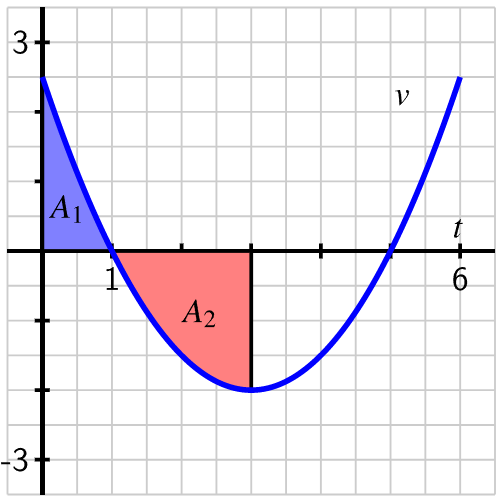
\includegraphics[width=0.3\textwidth]{images/fig-5-1-5.png}
\hfill
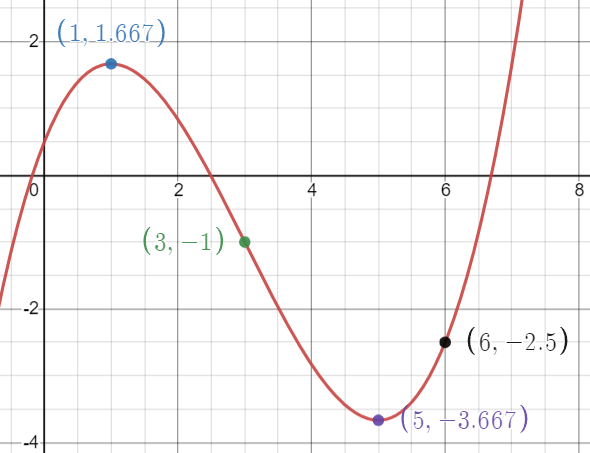
\includegraphics[width=0.35\textwidth]{images/fig-5-1-5-d.png}

\begin{enumerate}
    \item Use the given information to determine $s(1)$, $s(3)$, $s(5)$, and $s(6)$.
    
    \begin{red}
    {\everymath{\displaystyle}
    $s(1) = s(0) + \int_0^1 v(t)\, dt$, and $\int_0^1 v(t)\, dt = A_1$, so $s(1) = 0.5 + \frac{7}{6} = \frac53$.
    
    $s(3) = s(1) + \int_1^3 v(t)\, dt$, and that integral is $A_2$ except that it's going to count negative, so $s(3) = \frac53 - \frac83 = -1$.
    
    $s(5) = s(3) + \int_3^5 v(t)\, dt$. Because of symmetry, that integral is the same size as $A_2$, so $s(5) = -1 - \frac83 = -\frac{11}{3}$.
    
    $s(6) = s(5) + \int_5^6 v(t)\, dt$. Because of symmetry, that integral is the same size as $A_1$, so $s(6) = -\frac{11}{3} + \frac{7}{6} = -\frac52$.
    }
    \end{red}
    \item On what interval(s) is $s$ increasing? On what interval(s) is $s$ decreasing?
    
    \begin{red}
    $s$ is increasing wherever $v$ is positive, so on the intervals $[0, 1]$ and $[5,6]$.
    
    $s$ is decreasing wherever $v$ is negative, so on the interval $[1, 5]$.
    \end{red}
    
    \item On what interval(s) is $s$ concave up? On what interval(s) is $s$ concave down?
    
    \begin{red}
    $s$ is concave up wherever $v$ is increasing, so on the interval $[3,6]$.
    
    $s$ is concave down wherever $v$ is decreasing, so on the interval $[0,3]$.
    \end{red}
    
    \item Sketch an accurate, labeled graph of $s$.
    
    \begin{red}
    See above!
    \end{red}
    \item Note that $v(t) = -2 + \frac{1}{2}(t-3)^2$. Find a formula for $s$.
    
    \begin{red}
    $s$ is the antiderivative of $v$ such that $s(0) = 0.5$:
    \begin{align*}
        s(t) &= \int v(t)\, dt = \int -2 + \frac12 (t-3)^2\, dt \\
        \intertext{I'm going to sneakily do a $u$-substitution here with $u = t-3$.}
        &= -2t + \frac12 \cdot \frac13 (t-3)^3 + C \\
        0.5 = s(0) &= -2\cdot 0 + \frac16 (0-3)^3 + C \\
        \frac{1}{2} &= -\frac{27}{6} + C = -\frac{9}{2} +C \textrm{, so } C = 5 \\
        s(t) &= -2t + \frac16 (t-3)^3 + 5
    \end{align*}
    \end{red}
\end{enumerate}
\pagebreak

\item (\href{https://activecalculus.org/single/sec-5-2-FTC2.html#hnc}{Activity 5.2.3})
Suppose that $f(t) = \frac{t}{1+t^2}$, and $F(x) = \int_0^x f(t)\, dt$.
\begin{enumerate}
    \item (Plot a graph of $f(t)$.)
    
    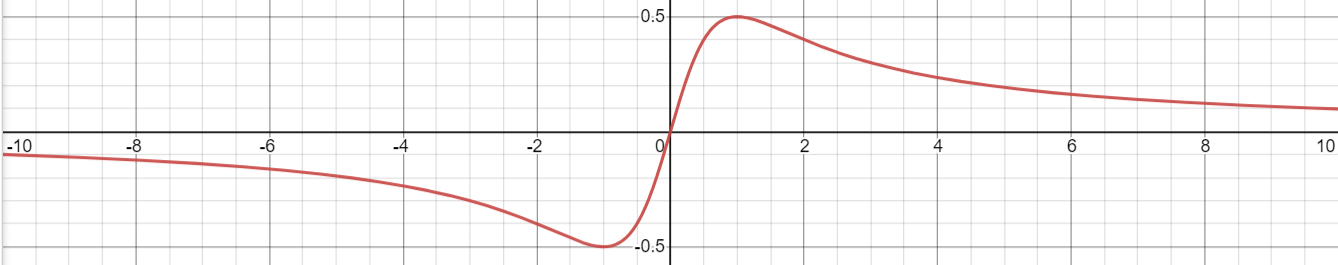
\includegraphics[width=0.95\textwidth]{images/fig-5-2-3-a.png}
    \item What is the key relationship between $F$ and $f$, according to the Second FTC?
    
    \begin{red}
    $F$ is an integral function, and according to the Second FTC, $F' = f$. That is, $f$ is the derivative of $F$.
    \end{red}
    \item Use the first derivative test to determine the intervals on which $F$ is increasing and decreasing.
    
    \begin{red}
    $F$ is increasing wherever $f$ is positive, so on the interval $[0, 10]$.
    
    $F$ is decreasing wherever $f$ is negative, so on the interval $[-10, 0]$.
    \end{red}
    \item Use the second derivative test to determine the intervals on which $F$ is concave up and concave down. Note that $f'(t)$ can be simplified to be written in the form $f'(t) = \dfrac{1-t^2}{(1+t^2)^2}$.
    
    \begin{red}
    Note first of all that since $F' = f$, $F'' = f'$, which is why we care about this nifty way to write $f'(t)$. Since the denominator is something squared, it's always positive, which means that the sign of $f'(t)$ is controlled exclusively by this numerator $1-t^2$.
    
    $F$ is concave up wherever $f'$ is positive, which is on the interval $[-1, 1]$. 
    
    $F$ is concave down wherever $f'$ is negative, which is on the intervals $[-10, -1]$ and $[1, 10]$.
    \end{red}
    \item Using technology appropriately, estimate the values of $F(5)$ and $F(10)$ through appropriate Riemann sums.
    
    \begin{red}
    I decided to use midpoint Riemann sums on Geogebra, with 10 rectangles for the first one and 20 rectangles for the second one. Here's the commands I used (after defining $f(t)$ appropriately, of course):
    
    \texttt{RectangleSum(f,0,5,10,0.5)} gave me that $F(5) = \int_0^5 f(t)\, dt \approx 1.6404$.
    
    \texttt{RectangleSum(f,0,10,20,0.5)} gave me that $F(10) = \int_0^{10} f(t)\, dt \approx 2.3186$.
    
    Your numbers may of course be a little different from mine, depending on how you did your Riemann sums.
    \end{red}
    \item Sketch an accurate graph of $y=F(x)$.
    
    \begin{red}
    I labeled some points on here including the inflection points and the two values from part (c).
    \end{red}
    
    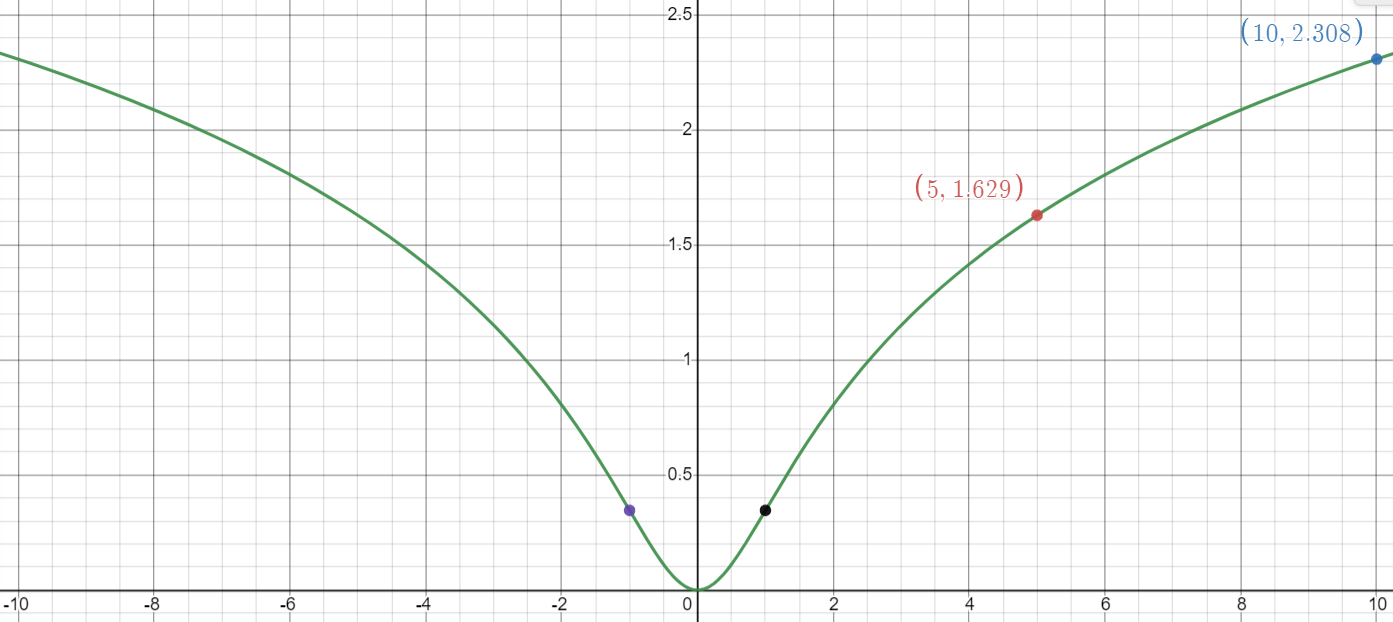
\includegraphics[width=0.95\textwidth]{images/fig-5-2-3-f.png}
 
\end{enumerate}
\end{enumerate}
\end{document}